%%%%%%%%%%%%%%%%%%%%%%%%%%%%%%%%%%%%%%%%%%%%%%%%%%%%%%%%%%%%%

\mainmatter
\setcounter{page}{1}

\lectureseries[\course]{\course}

\auth[\lecAuth]{Lecturer: \lecAuth\\ Scribe: \scribe}
\date{February 2, 2010}

\setaddress

% the following hack starts the lecture numbering at 1
\setcounter{lecture}{8}
\setcounter{chapter}{8}

\lecture{Quadratic Forms \& Attraction}

\section{Quadratic Forms}
Let $V(x)=x^TPx$. This gives $V$ pdf $\Leftrightarrow P>0 \Leftrightarrow \lambda(P)>0$ implying that the leading principal minors test of $P>0$. The leading principal minors test works well by hand for systems up to order $n=3$. For this type of quadratic system is $\dot{V}<0$? Consider $\dot{x}=Ax$ and see that $x=0$ is a.s. if and only if there exists $P=P^T$, $P>0$ such that $PA+A^TP<0$.

\begin{example}
\begin{align*}
\left[\begin{array}{c c} 1 & 1 \\ 1 & 2 \end{array}\right]>0
\end{align*}
The first principal minor is $1$ and the second principal minor is the matrix determinant.
$\lozenge$
\end{example}

\begin{example}
\begin{align*}
\left[\begin{array}{c c} 1 & 2 \\ 2 & 2 \end{array}\right]\not\geq0
\end{align*}
The first principal minor is $1$ and the second principal minor is the matrix determinant.
$\lozenge$
\end{example}

\begin{example}
\begin{align*}
\left[\begin{array}{c c} 1 & \sqrt{2} \\ \sqrt{2} & 2 \end{array}\right]\geq0
\end{align*}
$\lozenge$
\end{example}

\section{Region of Attraction}
Figure ?? shows an unstable limit cycle with an equilibrium point at $x=0$. The interior of the limit cycle is the region of attraction.

Figure ?? shows a system with three equilibria where $x=0$ is a stable equilibrium and the other two equilibria are unstable saddle points. The bold curves are known as \textit{separatrices} and the region of attraction (ROA) is located between those two curves.

\begin{example}
Consider a pendulum with friction with dynamics given by
\begin{align*}
\dot{x}_1 &= x_2 \\
\dot{x}_2 &= -\tfrac{g}{l}\sin(x_1) - \tfrac{k}{m}x_2
\end{align*}
For the Lyapunov function the total energy of the system can be used:
\begin{align*}
\dot{V}_1(x) = \underbrace{\tfrac{g}{l}(1-cos(x_1))}_{\text{potential}} + \underbrace{\tfrac{1}{2}x_2^2}_{\text{kinetic}}
\end{align*}
\begin{itemize}
\item Is $V_1(x)>0$? Yes.
\item Is $\dot{V}_1(x)<0$? $\dot{V}_1(x) = -\tfrac{k}{m}x_2^2 \Rightarrow \dot{V}_1(x)\leq0$. Almost, only nsdf.
\item $x_2=0$ when the pendulum is changing directions. Recall that Lyapunov stability theorem just says that systems are stable/a.s. but does not say that systems are unstable. Since we know that the system is a.s. and $V_1(x)$ does not show this we need to find a better candidate Lyapunov function.
\end{itemize}

\begin{figure}[ht!]
	\centering
	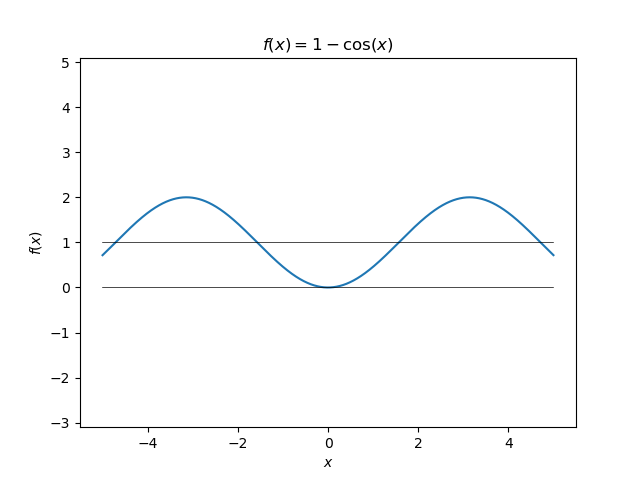
\includegraphics[width=.5\textwidth]{images/plot1minusCosX}
	\caption{Pendulum.}
	\label{fig:plot1minusCosX}
\end{figure}

Figure \ref{fig:plot1minusCosX} shows the function $f(x) = 1-\cos(x_1)$. The second Lyapunov function to try will be set up to take advantage of compeleting the squares.
\begin{align*}
V_2(x) &= V_1(x) + \tfrac{1}{2}\tfrac{k}{m}x_1x_2 + \tfrac{1}{4}\tfrac{k^2}{m^2}x_1^2 \\
&= \tfrac{g}{l}(1-\cos(x_1)) + \underbrace{\tfrac{1}{4}x_2^2 + \tfrac{1}{4}(x_2+\tfrac{k}{m}x_1)^2}_{<0}
\end{align*}
This gives $V_2>0$ on $D=(-\pi,\pi)\times\mathbb{R}$. Evaluating the derivative shows that
\begin{align*}
\dot{V}_2 = -\tfrac{1}{2}\tfrac{k}{m}x_2^2 - \tfrac{1}{2}\tfrac{g}{l}\tfrac{k}{m}x_1\sin(x_1) < 0
\end{align*}
on $D=(-\pi,\pi)\times\mathbb{R}$. Therefore $x=\left(\begin{array}{c} 0 \\ 0 \end{array}\right)$ is a.s. Now we want to look at the level sets that are generated by this system in Figure ??. Note that the ellipse inside the separatrices is the largest level set of $V_2$ and that \textsc{Matlab} can be used to find the level sets.
$\lozenge$
\end{example}

%%%%%%%%%%%%%%%%%%%%%%%%%%%%%%%%%%%%%%%%%%%%%%%%%%%%%%%%%%%%%
